\subsubsection{ Return paths}
After a {\dtop} has assembled, we know that the geometry the allows for the {\warpunit} to
work has been placed, therfore the counter is free to return back near where it started
reading the previous digit. The next gadget that assembles is the {\returnpath} gadget.
The basic idea of this gadget is simply to provide a path from the end of {\dtop} to some
general area closer to where the most recently read digit is located. Once the {\returnpath} has
completely assembled, it output's a glue for the {\nextread} gadgets to determine
where the counter needs to assemble next.


For each $\inc\in \{ {\tt increment}, {\tt copy} \}$:

\begin{itemize}

    % DIGIT 1
    \item Create
    $\begin{aligned}[t]
        \returnpath(& \left\langle {\tt ReturnPath}, 1, \inc \right\rangle,
                      \left\langle {\tt NextRead},   1, \inc \right\rangle \;)
    \end{aligned}$\\from the general gadget shown in Figure~\ref{fig:return_path_1_op}.

    \item Create
    $\begin{aligned}[t]
        \returnpath(& \left\langle {\tt ReturnPath}, 1, \inc, {\tt msr} \right\rangle,
                      \left\langle {\tt NextRead},   1, \inc, {\tt msr} \right\rangle \;)
    \end{aligned}$\\from the general gadget shown in Figure~\ref{fig:return_path_1_op_msr}

    \item Create
    $\begin{aligned}[t]
        \returnpath(& \left\langle {\tt ReturnPath}, 1, \inc, {\tt msr}, {\tt msd} \right\rangle,
                      \left\langle {\tt NextRead},   1, \inc, {\tt msr}, {\tt msd} \right\rangle \;)
    \end{aligned}$\\from the general gadget shown in Figure~\ref{fig:return_path_1-or-2_op_msr_msd}.


    % DIGIT 2
    \item Create
    $\begin{aligned}[t]
        \returnpath(& \left\langle {\tt ReturnPath}, 2, \inc \right\rangle,
                      \left\langle {\tt NextRead},   2, \inc \right\rangle \;)
    \end{aligned}$\\from the general gadget shown in Figure~\ref{fig:return_path_2_op-or-seed}.

    \item Create
    $\begin{aligned}[t]
        \returnpath(& \left\langle {\tt ReturnPath}, 2, \inc, {\tt msr}, {\tt msd} \right\rangle,
                      \left\langle {\tt NextRead},   2, \inc, {\tt msr}, {\tt msd} \right\rangle \;)
    \end{aligned}$\\from the general gadget shown in Figure~\ref{fig:return_path_1-or-2_op_msr_msd}.


    % DIGIT 3
    \item Create
    $\begin{aligned}[t]
        \returnpath(& \left\langle {\tt ReturnPath},  3, \inc \right\rangle,
                      \left\langle {\tt NextRead},    3, \inc \right\rangle \;)
    \end{aligned}$\\from the general gadget shown in Figure~\ref{fig:return_path_3}.


    \item Create
    $\begin{aligned}[t]
        \returnpath(& \left\langle {\tt ReturnPath}, 3, \inc, {\tt msr}, {\tt msd} \right\rangle,
                      \left\langle {\tt NextRead},   3, \inc, {\tt msr}, {\tt msd} \right\rangle \;)
    \end{aligned}$\\from the general gadget shown in Figure~\ref{fig:return_path_3}.

\end{itemize}

\begin{figure}[H]
    \centering
    \subcaptionbox{
        Digit 1 - general.
        \label{fig:return_path_1_op}
    }{\makebox[0.24\textwidth][c]{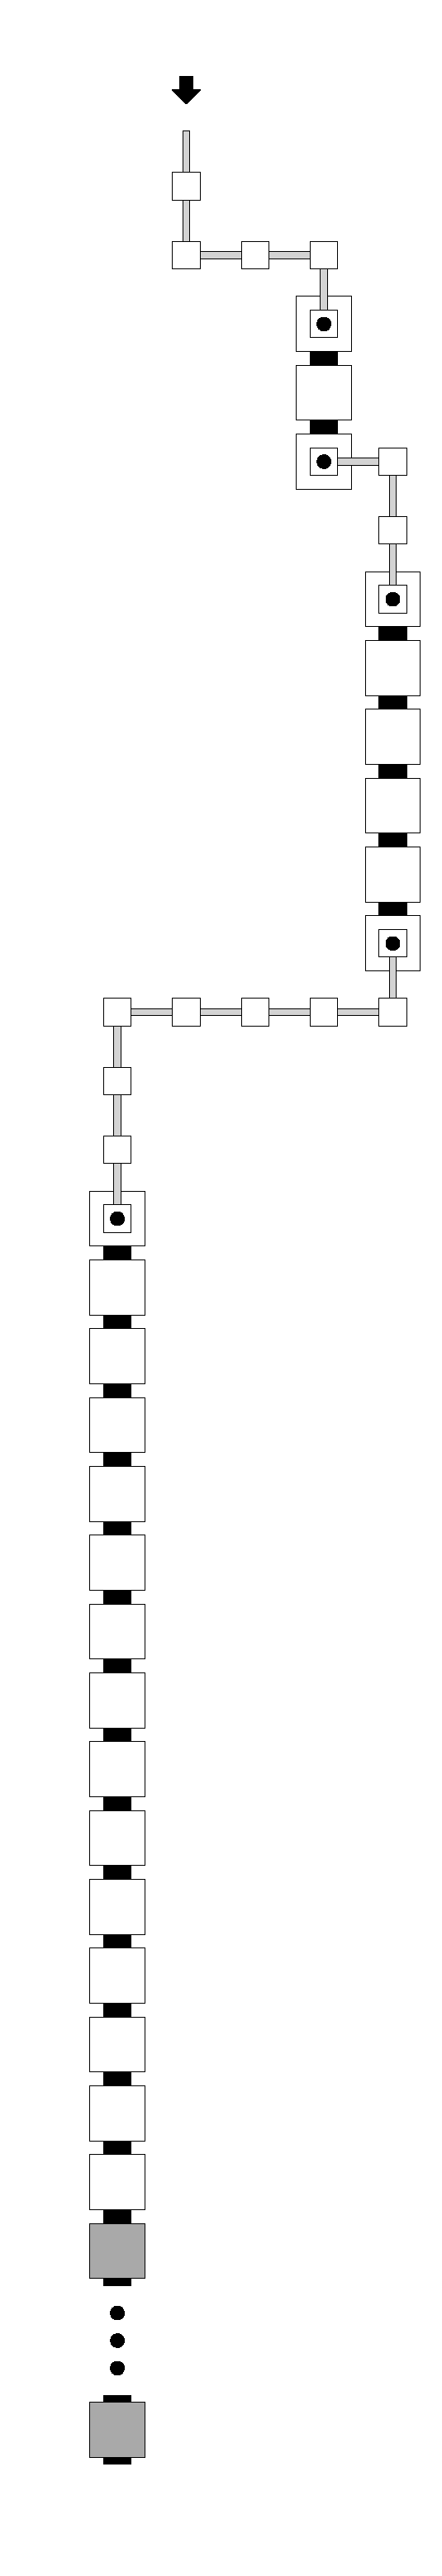
\includegraphics[width=0.45in]{return_path_1_op}}}%
    ~
    \subcaptionbox{
        Digit 1 - general\\overview.
        The black tiles in this figure correspond to the gadget shown in subfigure~\subref{fig:return_path_1_op}.
        \label{fig:return_path_1_op_overview}
    }{\makebox[0.24\textwidth][c]{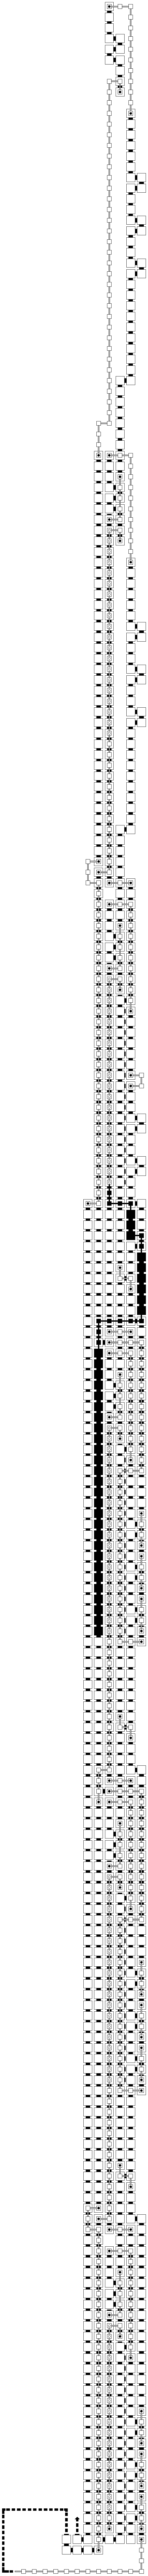
\includegraphics[width=0.45in]{overviews/general/return_path_1_op}}}%
    ~
    \subcaptionbox{
        Digit 1 - general (seed) overview.
        The black tile in this figure is a single tile gadget used only in the initial value.
        \label{fig:return_path_1_seed_op_overview}
    }{\makebox[0.24\textwidth][c]{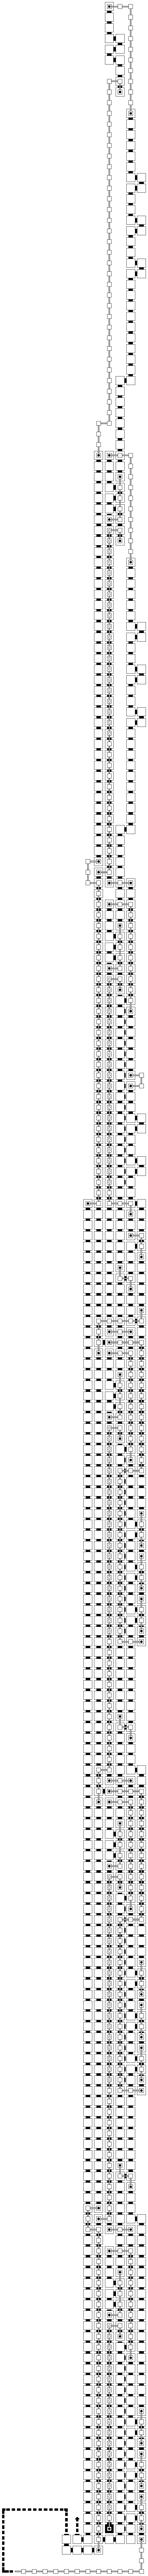
\includegraphics[width=0.45in]{overviews/general/return_path_1_seed_op}}}%
    ~
    \subcaptionbox{
        Digit 2 - general.
        \label{fig:return_path_2_op-or-seed}
    }{\makebox[0.24\textwidth][c]{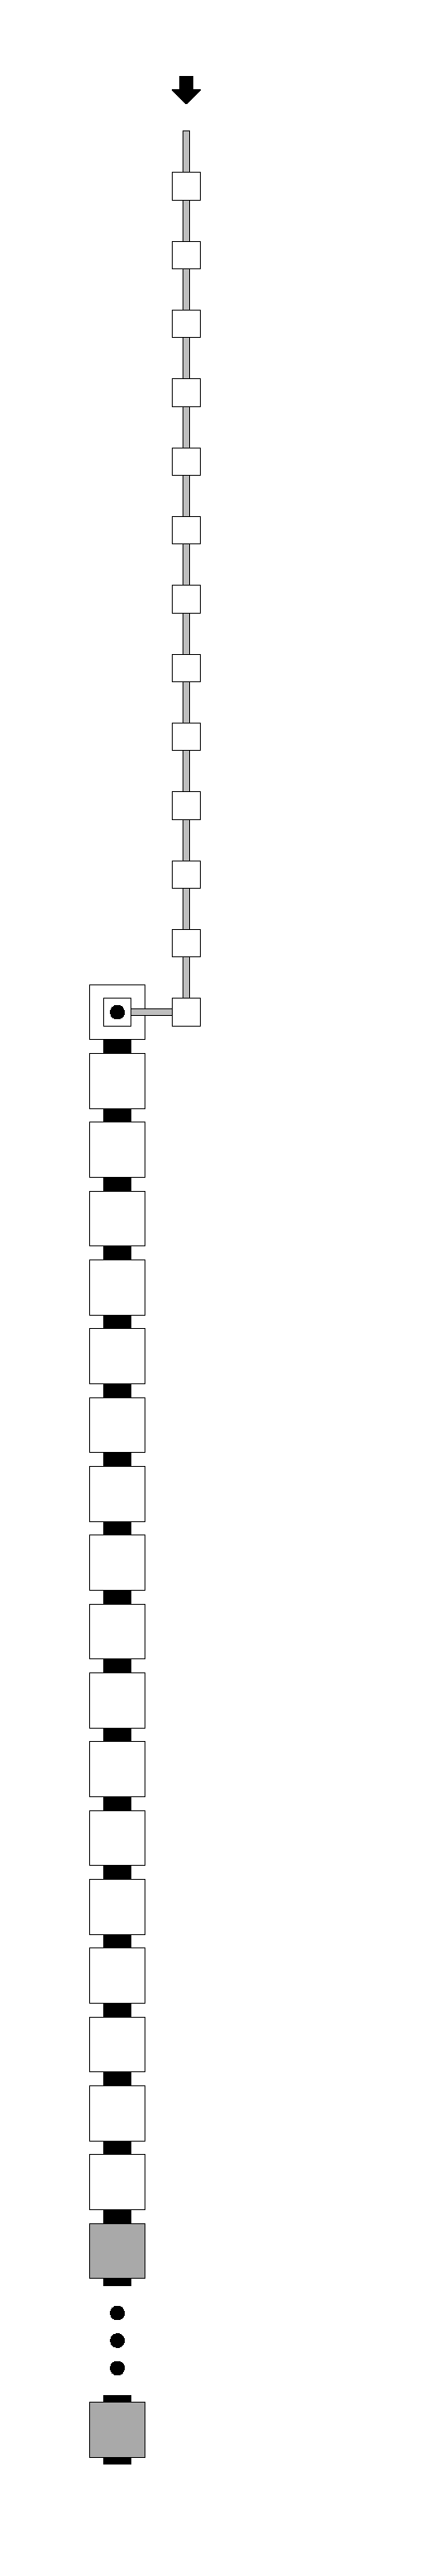
\includegraphics[width=0.45in]{return_path_2_op-or-seed}}}%
    ~
\end{figure}
\begin{figure}[H]\ContinuedFloat
    \centering
    \subcaptionbox{
        Digit 2 - general\\overview.
        The black tiles in this figure correspond to the gadget shown in subfigure~\subref{fig:return_path_2_op-or-seed}.
        \label{fig:return_path_2_op_overview}
    }{\makebox[0.24\textwidth][c]{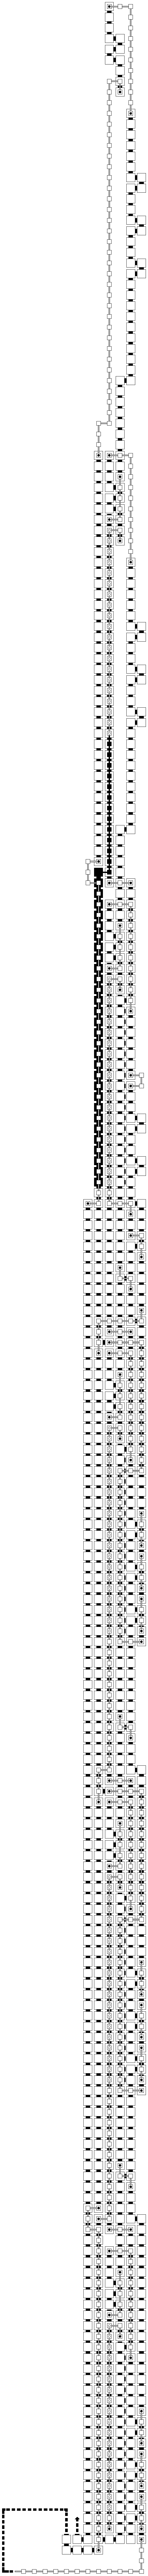
\includegraphics[width=0.45in]{overviews/general/return_path_2_op}}}%
    ~
    \subcaptionbox{
        Digit 2 - general (seed) overview.
        The black tiles in this figure correspond to the gadget shown in subfigure~\subref{fig:return_path_2_op-or-seed}.
        \label{fig:return_path_2_seed_op_overview}
    }{\makebox[0.24\textwidth][c]{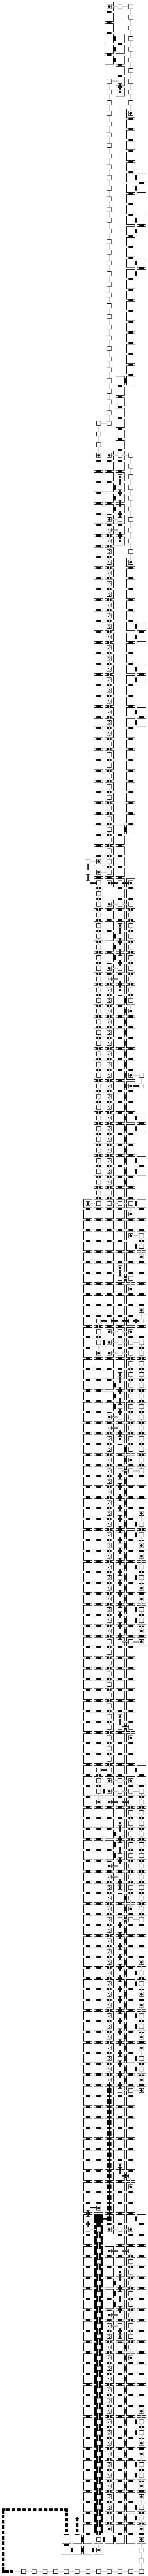
\includegraphics[width=0.45in]{overviews/general/return_path_2_seed_op}}}%
    ~
    \subcaptionbox{
        Digit 3 - general.
        \label{fig:return_path_3}
    }{\makebox[0.24\textwidth][c]{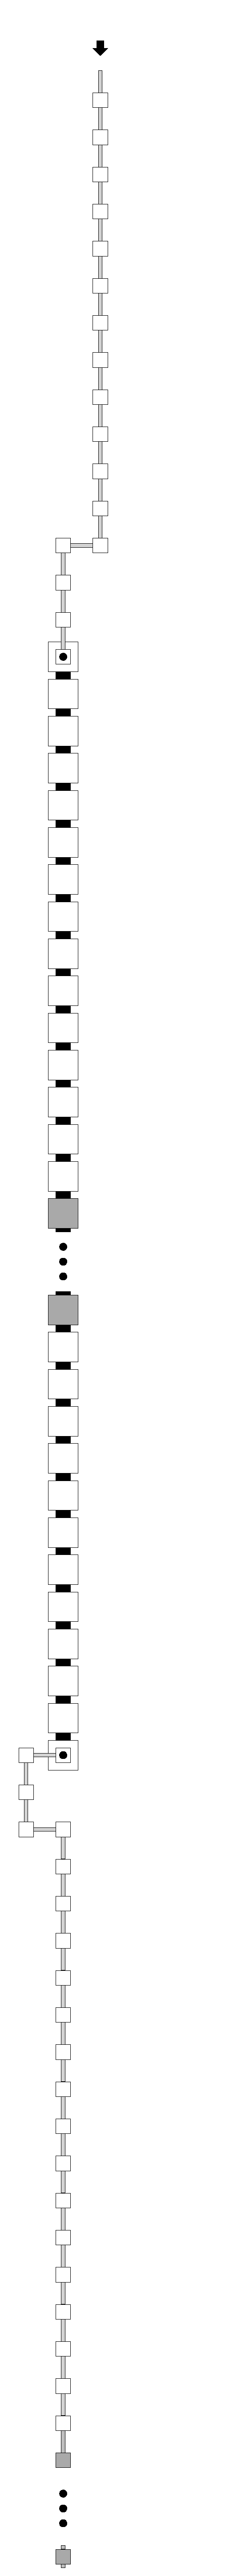
\includegraphics[width=0.45in]{return_path_3}}}%
    ~
    \subcaptionbox{
        Digit 3 - general\\overview.
        The black tiles in this figure correspond to the gadget shown in subfigure~\subref{fig:return_path_3}.
        \label{fig:return_path_3_op_overview}
    }{\makebox[0.24\textwidth][c]{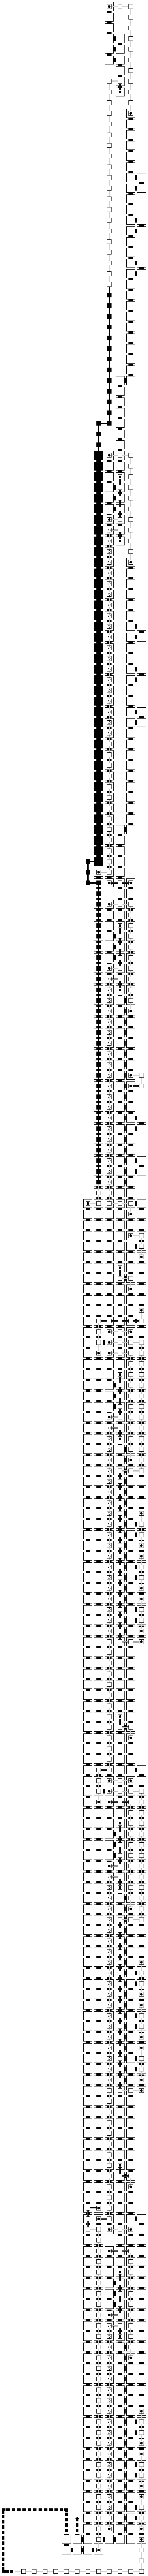
\includegraphics[width=0.45in]{overviews/general/return_path_3_op}}}%
    ~
\end{figure}
\begin{figure}[H]\ContinuedFloat
    \centering
    \subcaptionbox{
        Digit 3 - general (seed) overview.
        The black tiles in this figure correspond to the gadget shown in subfigure~\subref{fig:return_path_3}.
        \label{fig:return_path_3_seed_op_overview}
    }{\makebox[0.24\textwidth][c]{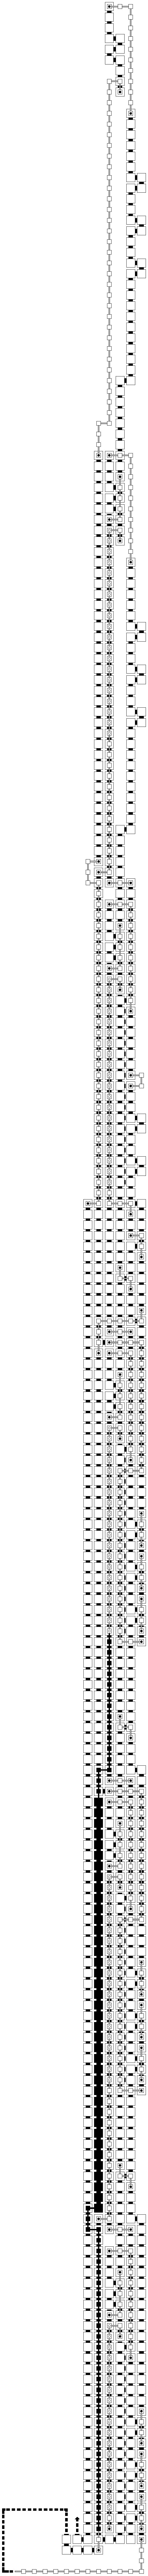
\includegraphics[width=0.45in]{overviews/general/return_path_3_seed_op}}}%
    ~
    \subcaptionbox{
        Digit 1 - case 2.
        \label{fig:return_path_1_op_msr}
    }{\makebox[0.24\textwidth][c]{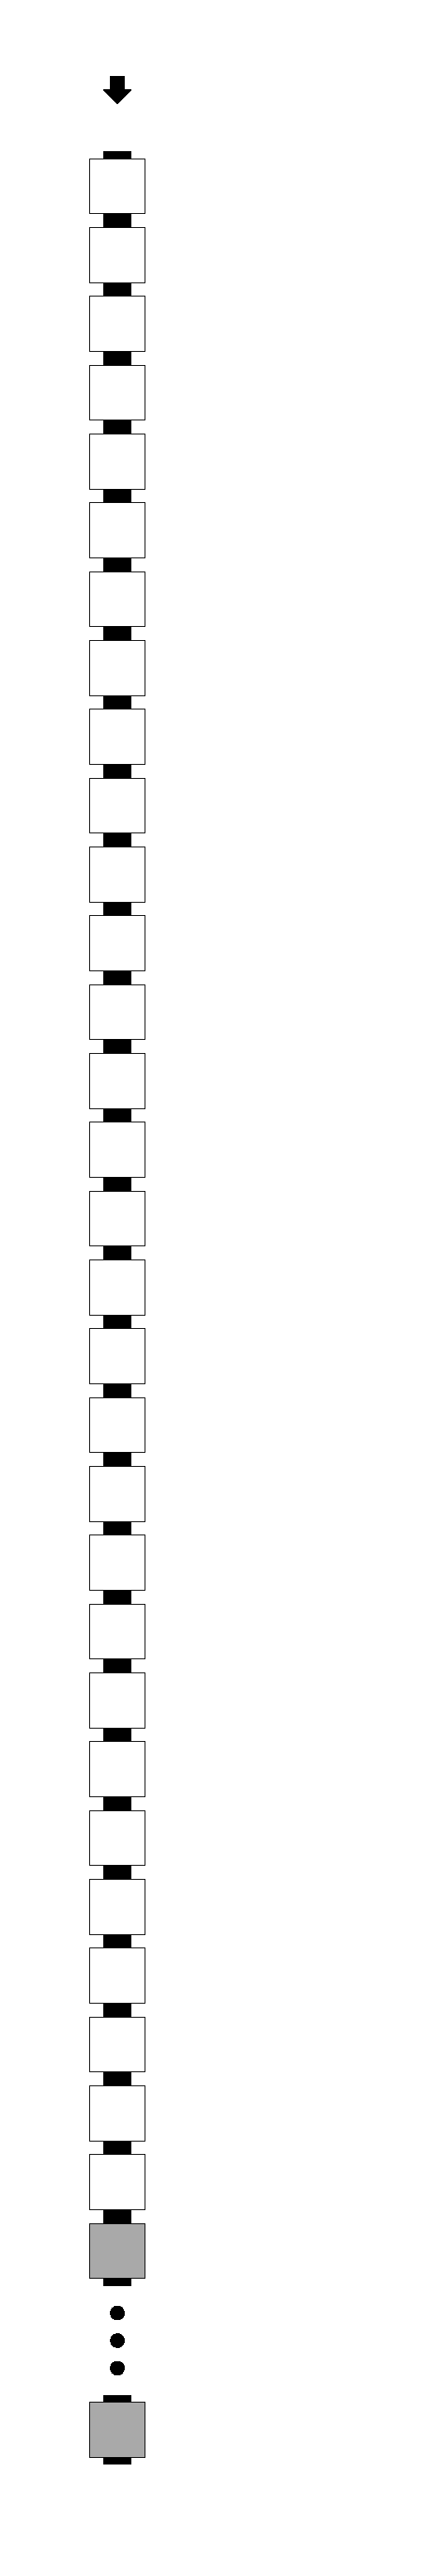
\includegraphics[width=0.45in]{return_path_1_op_msr}}}%
    ~
    \subcaptionbox{
        Digit 1 - case 2 overview.
        The black tiles in this figure correspond to the gadget shown in subfigure~\subref{fig:return_path_1_op_msr}.
        \label{fig:return_path_1_op_msr_overview}
    }{\makebox[0.24\textwidth][c]{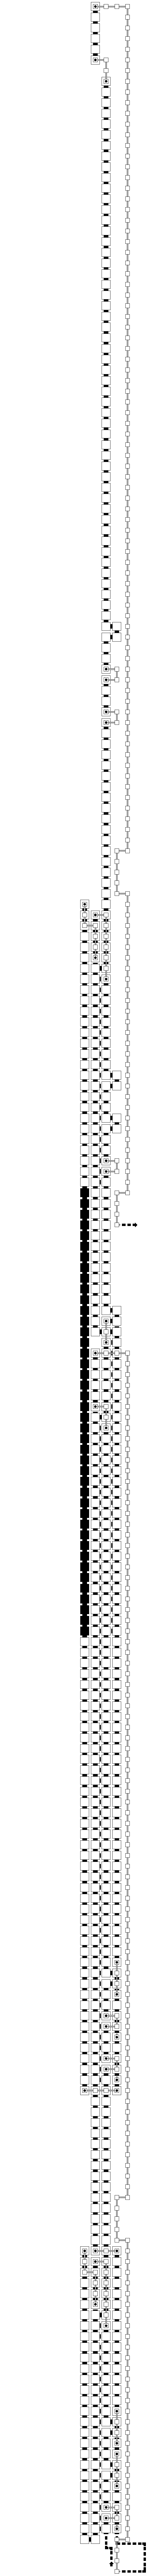
\includegraphics[width=0.45in]{overviews/case2/return_path_1_op_msr}}}%
    ~
    \subcaptionbox{
        Digit 1 - case 2 (seed) overview.
        The black tile in this figure is a single tile gadget used only in the initial value.
        \label{fig:return_path_1_seed_op_msr_overview}
    }{\makebox[0.24\textwidth][c]{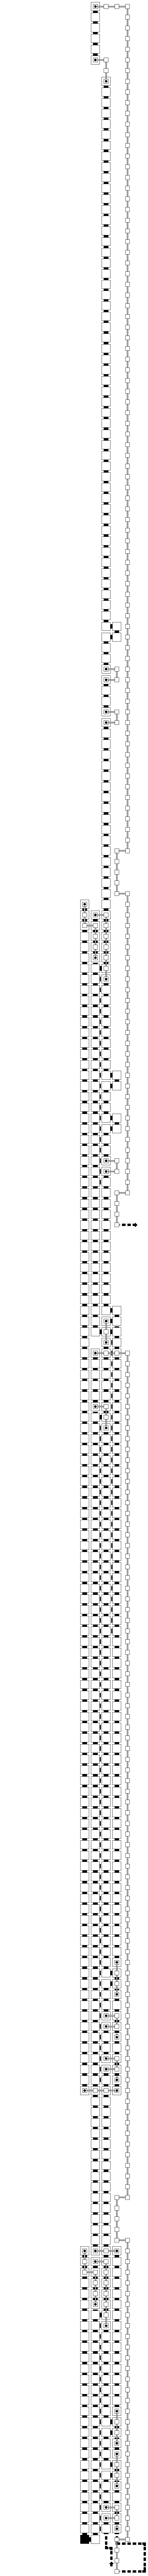
\includegraphics[width=0.45in]{overviews/case2/return_path_1_seed_op_msr}}}%
    ~
\end{figure}
\begin{figure}[H]\ContinuedFloat
    \subcaptionbox{
        Digit 1 - case 1,\\Digit 2 case 2.
        \label{fig:return_path_1-or-2_op_msr_msd}
    }{\makebox[0.24\textwidth][c]{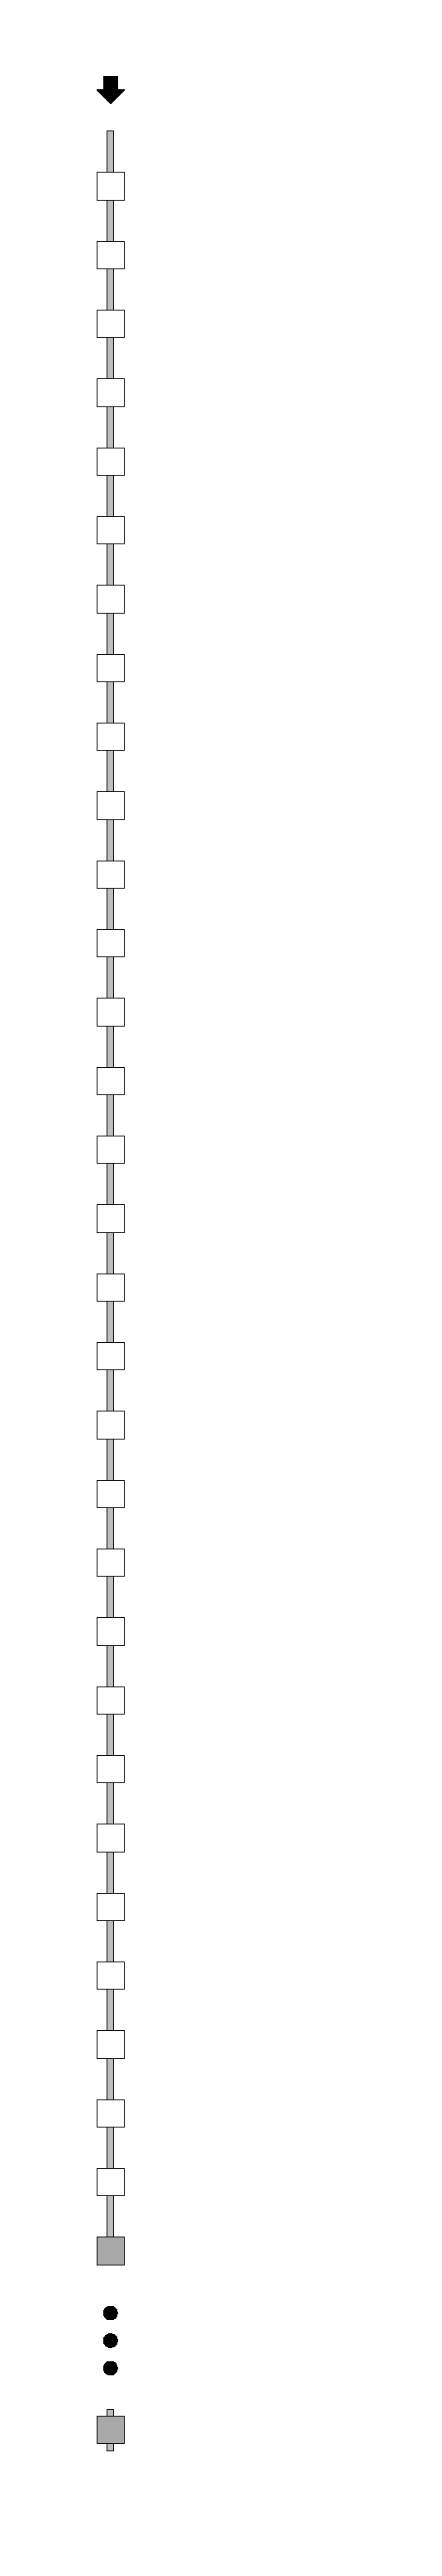
\includegraphics[width=0.45in]{return_path_1-or-2_op_msr_msd}}}%
    ~
    \subcaptionbox{
        Digit 1 - case 1 overview.
        The black tiles in this figure correspond to the gadget shown in subfigure~\subref{fig:return_path_1-or-2_op_msr_msd}.
        \label{fig:return_path_1_op_msr_msd_overview}
    }{\makebox[0.24\textwidth][c]{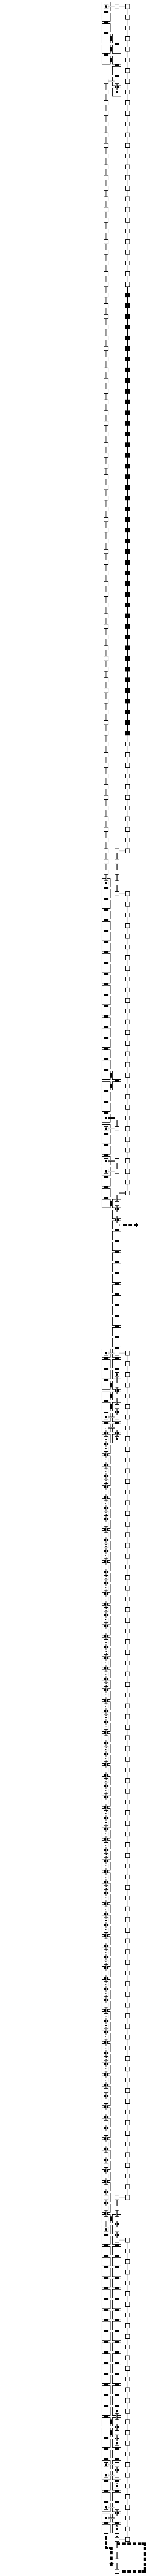
\includegraphics[width=0.45in]{overviews/case1/return_path_1_op_msr_msd}}}%
    ~
    \subcaptionbox{
        Digit 1 - case 1 (seed) overview.
        The black tiles in this figure correspond to the gadget shown in subfigure~\subref{fig:return_path_1-or-2_op_msr_msd}.
        \label{fig:return_path_1_seed_op_msr_msd_overview}
    }{\makebox[0.24\textwidth][c]{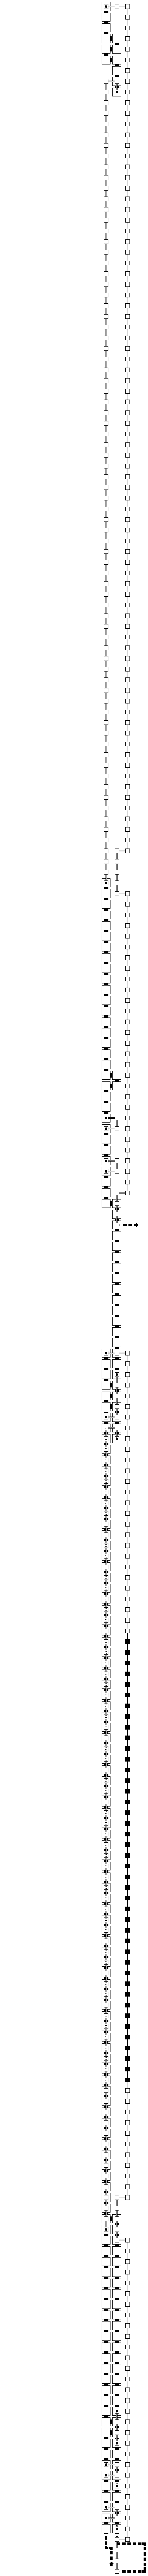
\includegraphics[width=0.45in]{overviews/case1/return_path_1_seed_op_msr_msd}}}%
    ~
    \subcaptionbox{
        Digit 2 - case 2 overview.
        The black tiles in this figure correspond to the gadget shown in subfigure~\subref{fig:return_path_1-or-2_op_msr_msd}.
        \label{fig:return_path_2_op_msr_msd_overview}
    }{\makebox[0.24\textwidth][c]{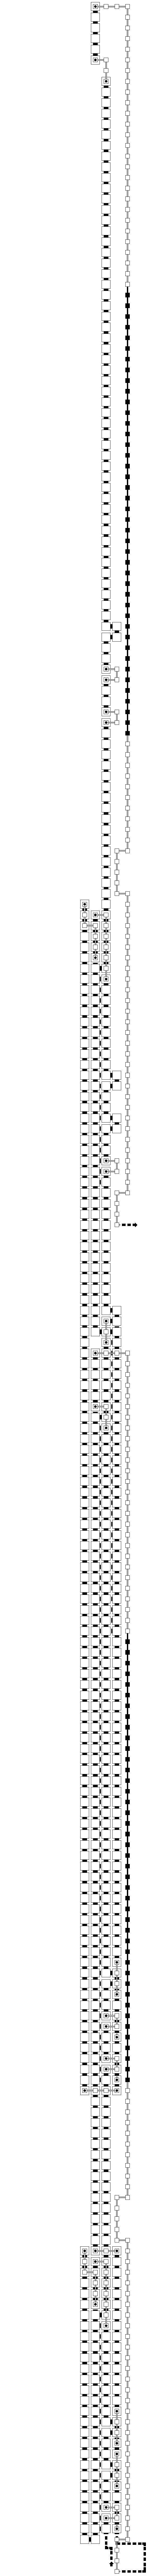
\includegraphics[width=0.45in]{overviews/case2/return_path_2_op_msr_msd}}}%
    ~
    \caption{\label{fig:return_path_gadgets} The {\tt Return\_Path} gadgets.}
\end{figure}
\begin{figure}[H]\ContinuedFloat
    \centering
    \subcaptionbox{
        Digit 3 - case 3 overview.
        The black tiles in this figure correspond to the gadget shown in subfigure~\subref{fig:return_path_3}.
        \label{fig:return_path_3_op_msr_msd_overview}
    }{\makebox[0.24\textwidth][c]{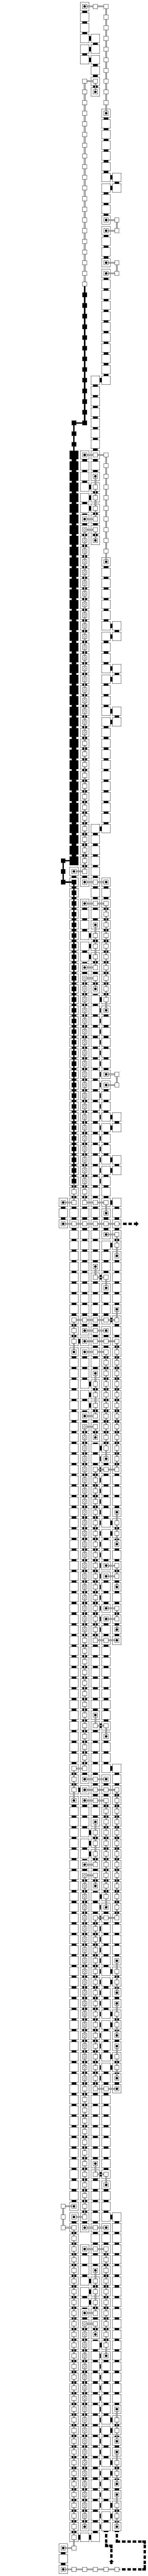
\includegraphics[width=0.45in]{overviews/case3/return_path_3_op_msr_msd}}}%
    ~
    \subcaptionbox{
        Digit 3 - case 3 (seed) overview.
        The black tiles in this figure correspond to the gadget shown in subfigure~\subref{fig:return_path_3}.
        \label{fig:return_path_3_seed_op_msr_msd_overview}
    }{\makebox[0.24\textwidth][c]{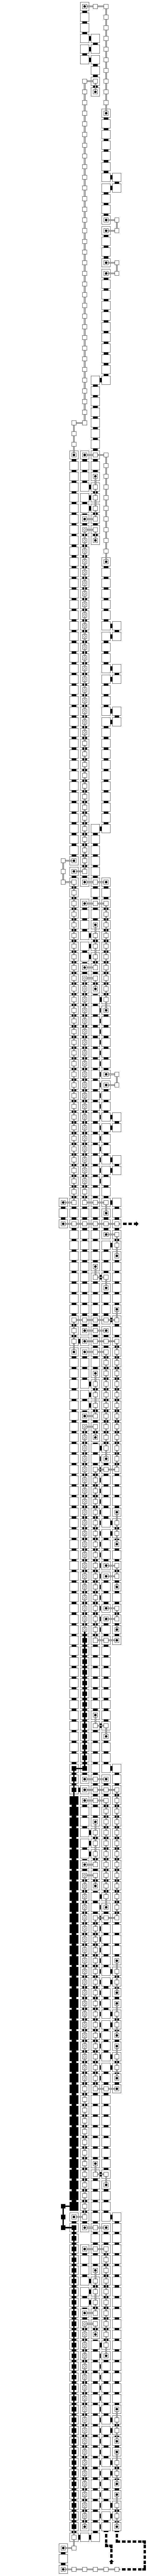
\includegraphics[width=0.45in]{overviews/case3/return_path_3_seed_op_msr_msd}}}%
    ~
\end{figure}

